\documentclass{article}
\usepackage[utf8]{inputenc}
\usepackage[a4paper, margin=1in]{geometry}
\usepackage[font={small,it}]{caption}
\usepackage{graphicx}
\usepackage{xcolor}
\usepackage{pdfpages}
\usepackage{natbib}
\usepackage{graphicx}
\usepackage{float}
\usepackage{url}
\usepackage{nameref}
\usepackage{pdflscape}
\usepackage{listings}
\usepackage{xparse}
\usepackage{hyperref}

\graphicspath{{../Figures/}}
\bibliographystyle{agsm}
\NewDocumentCommand{\codeword}{v}{%
\texttt{{#1}}%
}
\lstset{language=C,keywordstyle={\bfseries}}
\hypersetup{
    colorlinks,
    citecolor=black,
    filecolor=black,
    linkcolor=black,
    urlcolor=black
}

\title{\textbf{Examining the Usage of Advanced Programming Constructs}}
\author{
Luca Davies \\ M.Sci. (Hons.) Computer Science (with Industrial Experience)}
\date{4th June 2021}

\begin{document}
\maketitle

\newpage
\section*{Declaration}
    I certify that the material contained in this dissertation is my own work and does not contain unreferenced or unacknowledged material. I also warrant that the above statement applies to the implementation of the project and all associated documentation. Regarding the electronically submitted work, I consent to this being stored electronically and copied for assessment purposes, including the School’s use of plagiarism detection systems in order to check the integrity of assessed work. \\
    I agree to my dissertation being placed in the public domain, with my name explicitly included as the author of the work. \\
    
    \noindent
    Name: Luca Davies\\
    Date: 01/06/2021
\newpage
\section*{Abstract}
    As time has gone on, languages have become more developed themselves more advanced syntax constructs have been added alongside many "quality of life" type structures to make the writing code not only more efficient but also easier for developers. This report examines seven of these advanced constructs, drawing together both data from surveys taken by professional developers and data from analysis of a four widely known, active, open source code bases. Using a short but broad survey, data was collected on developers' usage of these constructs and they provided information on how they felt these constructs affected their code and how often they used them, and how they thought they existed within the context of the wider industry. Analysis of code was carried using a combination of both simple regular expressions and via the user of lightweight tool to aid in the bulk processing of a large volume of source code file. It was found that ... don't know yet. FINISH ABSTRACT WITH RESULTS.
    \newline
    \newline
    [Is there any working docs?]
\newpage
\tableofcontents

\newpage
\section{Introduction}
    \subsection{Overview}
    \label{sec:overview}
        Code style has long been a topic of heated debated within the field of computer science since even the very early days. You will rarely ever get a single consensus in room when asking ``How should code blocks be indented?'', or worse still ``What is the best brace style?''. These kinds of physical layout questions have been around as long as the languages they exist within, but as programming languages have become more complex and afford programmers greater ease to express their logic, this discussion of best style has only broadened. Languages include more `syntactic sugar' constructs, patterns and operators that allow the simplification of previously more complex-looking or verbose statements. Such constructs and operators as:

        \begin{itemize}
            \item Ternary/in-line If Statements ( \codeword{a ? b : c} )
            \item Null-coalesce ( \codeword{a ?? b} ) and Null-conditional Operators ( \codeword{a?.b} / \codeword{a?[x]b})
            \item Lambda Expressions and Anonymous Functions ( \codeword{(a) => { b; }} )
            \item Additional constructs:
            \begin{itemize}
                \item Foreach Loops ( \codeword{foreach (a in b)} / \codeword{for ( a : b )})
                \item Unary Increment Operators (\codeword{a++}, \codeword{b--})
                \item Compound Assignment Operators (\codeword{a += 2},  \codeword{b -= 2}, \codeword{c *= 2}, \codeword{d /= 2}, etc...)
            \end{itemize}
        \end{itemize}
        
        \emph{Detailed descriptions of these constructs are given in Section \ref{subsec:constructs}}\\

        Prior to this project, I was working on a large C\# codebase with a nearly 20 year history. Throughout that time, the notion of `ideal' style had changed not only within the company the codebase belonged to, but in the wider software industry too. This led to wide mix of `plain' (or without syntactic sugar-like statements) together with many of the newer syntax constructs. For example, lambdas were only added to C\# around seven or eight \emph{years} after the first iteration of the codebase had been written. Some files featured a complete lack of any of these more advanced syntax constructs, some had many, some had some very painful to read examples of their use, where perhaps it may have been better to have used more traditional syntax. It is this mix-and-match of the use of these constructs that spurred the idea of this project. Looking at code, there are clearly times when traditional syntax is overly verbose and takes up more space on the screen than necessary, but it also became abundantly clear that to swap out \emph{all} plain syntax for these more compact styles would be a big mistake, making many bits of code much harder to read.

        So where does the line lie between when to, and when to not use these constructs? To answer this, we must consider why we would use either one or the other at all. Often they are used to make code more compact - as software development has grown as an industry, there are certain `set' statements that it can generally be assumed that everyone understands, and that can be abstracted a little to make them neater or smaller. Other times it may be what has been laid out in a company style guide that everyone should use, or perhaps purely the habits and practices of an individual. However, regardless of the exact reason or motivation behind every use of these constructs, it is important to remember that no tool is unable to be misused - overuse of these types of constructs or use of them in inappropriate places, can make code more complicated and harder to read than it would have been otherwise. It is equally important to value the `plain' or verbose syntax as much as the compact variants, both having very unique and distinct advantages and disadvantages.
        \\

        This project began with an aim to make recommendations on how to best use the constructs in question, but as research continued and it was found just how little clear guidance is available, and how much conflict and indecision is present, it has become a more exploratory study in the use and usage of theses constructs. To do so, we focus on C\#, JavaScript, and Java as a representative sample of popular imperative programming languages.

        They may be used for multiple reasons, such as to make code simpler, or clearer. Other times, it may be style defined either by a programmer themselves, or the house rules of their organisation.  In this paper, we will study the above constructs and how they are used, with a view to making recommendations about they are best used, and where they are best avoided.
    \subsection{Motivation}
        The primary drive for this study stems from my experience during my industrial placement (SCC.419). As briefly mentioned above, the codebase I was working on was extensive and developed by numerous developers over the course of the last two decades or so. There were times that code was either made easier or harder not by its flow, but by the way it was written. The first instance that came to my attention was a ternary if-statement used that was so long that it needed to be split across four lines, had a second and third ternary in the true \emph{and} false branch of the enclosing ternary, with lengthy expressions being evaluated from there. In this instance, it can be assumed that it would have been significantly clearer to use a regular if-statement. Despite this the existence of ternary if-statements is still useful, but it brings to question where these constructs and other similar constructs should best be used.

        There also seems to have been relatively little research into languages features such as these, either in terms of subjective readability or objective performance. Some studies I have come across in research even make explicit note of the fact their definition of `good style' is subjective and opinion-based, albeit from that of perceived experts. Using experts in a field is always a good sign, but if there really is very little guidance to any level of programmer, then it stands to reason that much of what even experts think is good style, could be from personal experience alone, or at least somewhat unacademic.
        
        It is hoped that by formally examining these constructs in an academic context that the produced research will a launch pad or grounding for more thorough examination across the software development industry as a whole.
    \subsection{Aims \& Objectives}
        The aims of this report are as follows:
        \begin{enumerate}
            \item To understand the usage of seven advanced programming constructs (as defined in sections \ref{sec:overview} and \ref{subsec:constructs})
            \item To study what reasons developers have to or to not use these constructs
            \item To make take the first steps in creating formal, unified recommendations on the use of these constructs 
        \end{enumerate}


        These aims will be achieved via the following objectives:
        \begin{enumerate}
            \item Collect data from professional developers about when and how they think it is appropriate to use these constructs via a survey
            \item Investigate what guidance is available to developers on how to use these constructs by examining available style documents provided by developers and online
            \item Examine the recommendations made by static code analysis tools on specifically written `control' code files
            \item Analyse four open source repositories to assess how these constructs are used in practice both by hand and using static code analysis tools
            \item Conduct profiling and performance tests of the constructs (stretch objective)
        \end{enumerate}

    \subsection{Methods}
        A multifaceted approached was taken to achieve the above aims, incorporating multiple methods. First, a survey was carried out, to gather both qualitative and quantitative data direct from developers about how they use each of the constructs being examined - this helps address aim one. A survey was chosen as it provides a comparatively easy method to gather answers to base questions from a large sample size.
        Quantitative data was collected, with regard to aim two, by employing static code analysis tools to analyse four open source GitHub repositories and `control' files (giving examples of both the constructs and their `plain' equivalents), in three programming languages. Static analysis tools were employed as they most likely represent actual tools developers may use to check their code, and thus the rules and recommendations that will be levelled against their code in a real scenario.
        Aims one and two were also supported by the analysis of the commit history of the aforementioned four repositories for changes that include or exclude the use of the constructs in question. Lastly, aim three will be met via a culmination of all methods used, and some simple numerical analysis.

        \subsubsection{Threats to Validity}
            Due to time constraints and limits of contacts, the survey was only able to encompass one group of programmers, all from within one company. Although the technology stack the developers in question may have been exposed to consisted primarily of C\# and JavaScript, this potentially means participants may have been answering questions with little knowledge on Java. The results of the survey are also difficult to generalise, as there are many factors which may affect responses that are limited to this one group of developers.

            The survey was distributed widely within ISS, giving approximately 60 potential respondents. Of those, there are 44recorded responses  (~70\% response rate), 23 of which are completed, valid responses (~40\% valid responses).
    \subsection{Report Structure}
        The remainder of this report will first detail further background research directly and indirectly related to this topic, before describing the methods and design of the study, followed by the results and information gained from the study, discussion on these results, before final conclusions.
\newpage
\section{Background}
\label{sec:background}
    At face-value, much of the grounding of this study may be considered conventional wisdom. That is, the constructs are simply used anywhere and everywhere according to when we as programmers deem it appropriate, without much prior thought or formal procedure. This once would have been the case for structural or physical style to our code, the way we lay our code out and arrange it around whitespace. Countless style guides have concerned themselves with this for many years, and there's still much debate around which brace style is the best in C-like languages, or how many spaces should be used to indent code blocks. It hasn't been until much more recent times, as software development houses have grown, and the computing industry as a whole has ballooned into the incredibly important sector it is today, that we have started to think more about the meta-style of our programming. Not how it's physically laid out, but how we layout our logic and design patterns. Somewhere between these two schools of thought lies the area this study is focussed on.

    It does not appear, however, that a great deal has been written and published around how to best use many of the programming constructs that many programmers will use tens, if not hundreds, of times per day. What follows is a summary of much of the existing works that cover partially on wholly the same topics.
    \subsection{Existing Literature}
        As far back as the 1980s, \cite{berryMeekingStyle} proposed the Berry-Meeking Style Metric as a measure of good style and readability of code. This used style analysers adapted specifically to C to produce a metric denoting the `lucidity' of the code. The metric was derived from 11 different characteristics about a program: module length, identifier length, percentage of comment lines, amount of indentation, percentage of blank lines, line length, spaces within lines, percentage of constants, reserved words used, included files and number of gotos used. Zooming out from this level of metric-based scoring, \cite{paradigmForStyleResearch} collects a number of studies of together and notes how application of these types of style metrics not only lack correlation with error proneness, but also has unpredictable effects on complexity metrics. They go further to say that style is an `intuitive and elusive' concept, that is `highly individualistic' and simultaneously easy to see, but hard to define. Many differing style guides are either too general or subjective, contradictory between each other and with no guidance and how to manage these conflicts. They go on to liken the use programming style to ``the `perception and judgement' a writer exercises in selecting `from equally correct expressions, the one the best suited to his material, audience and intention'{}''. This is to say that the nuance of writing in English prose is present too in the style of code.

        In more recent times, it is again reinforced that some simple metrics like program length cannot solely be used to measure the quality of code style. \cite{autoStyleFeedbackAtScale}, when showing a range of students' responses to a programming task (the shortest of which is unlikely to be rated the easiest to read), state that length is not a sole indicator of good style, and moreover that ``excessive terseness is often worse than that of verbosity''. We still don't have any \emph{definite} way to judge `good' style, with \cite{scaleDrivenHints} noting that their study on providing style hints to new programmers is limited by the fact the given `good' style is subjective and opinionated.

        One of the defining style guides for Java, Effective Java \citep{effectiveJava} makes many assertions about how to use certain features of the Java language, but most of these do not reach the level of granularity focussed on in this study. The reference to anything close is that Java programmers should ``prefer for-each loops over traditional for loops''. Lambdas feature in their own chapter, but only with reference to \emph{how} to use them, not \emph{when}.

        It is reasonable to think that official style guides published by programming language developers would be cover-all for all sorts of style, from the extraneous and finnicky to most basic syntax, but in fact, Microsoft's own style guide for C\# is somewhat short, and it's only relevant mention for this study being a note that lambdas are `shorter' and may thus be good substitutions for the more verbose regular methods that would be needed otherwise.

        Two prevailing style guides for JavaScript have come into prominence the last few years, both with certain small conflicts and differences from each other. These are the Google style JavaScript style guide \citep{googleJSStyle}, and the Airbnb JavaScript style guide \citep{airbnbJSStyle}. The Google guide advocate for use of \codeword{for-of} loops over all other types of \codeword{for} loop in JavaScript, allowing \codeword{for-in} loops exceptionally for dict-style objects. The Airbnb guide, conversely to Google, requires use of \emph{iterators} over \codeword{for-in} or \codeword{for-of}, with no reference to standard for loops. It also makes one very relevant assertion: that ternaries should ``not be nested and generally be single line expressions''. Perhaps controversially, the Airbnb guide also rejects the use of the unary operators, \codeword{++} and \codeword{--}. This is primarily due to the fact that these statement cause automatic semicolon insertion and can cause silent errors. However, it is also reasoned that the more expressive \codeword{+=} and \codeword{-=} operators allow code to be easier to read and less error-prone.
    \subsection{Constructs}
        \label{subsec:constructs}
        This section will give a more detailed description of each of the constructs to be examined. The constructs were selected for a number of reasons - firstly, they are all replaceable with simpler syntax (lambdas being a occasional exception, see Section \ref{subsubsec:lambdas}), conventional wisdom would dictate that some are rather commonly used (compound assignment / unary operators) and conversely that some are used much less (null-coalesce / null-conditional). Initial thoughts of some of the constructs came about from seeing then during my work for SCC.419. The constructs in question are detailed below:
        \newpage
        \begin{itemize}
            \item Ternary/in-line If Statements
                \begin{itemize}
                    \item Reduces the common \codeword{if} \dots \codeword{else} \dots pattern into a single line of the form \codeword{a ? b : c}, where \codeword{a} is a conditional expression, \codeword{b} is the body of the \codeword{if} and \codeword{c} is the body of the \codeword{else}. While it may be possible in some languages to have multiple statement in the `b' and `c' sections of a ternary, but standard syntax only permits a single statement.
                \end{itemize}
            \item Lambdas and Anonymous Functions
                \begin{itemize}
                    \item A lambda expression is any expression involving a function used as an argument, just as in Lambda Calculus. Though this is not required, lambdas most often take the form of anonymous (unnamed) functions defined in-line. \citep{javaLambdas}.
                \end{itemize}
            \item Null-coalescing Operator
                \begin{itemize}
                    \item Used to provide a default value in place of a null value. Replaces a null-check (using an if statement) with a single assignment of the form \newline\codeword{a = possiblyNullValue  ?? valueIfNull} where \codeword{a} is of a nullable type. \citep{cs5Spec}.
                \end{itemize}
            \item Null-conditional Operator
                \begin{itemize}
                    \item Used to access a member or element of its operand \emph{if and only if} that operand evaluates to non-null. Otherwise, it returns null. \citep{cs6Spec}. This allows a member/element access operation to be carried out without a null-check on the base operand, only on the evaluated value.
                \end{itemize}
             \item Foreach Loops
                \begin{itemize}
                    \item Used to simplify for loops for the purposes of iterating over an abstract data structure, usually a type of some form of collection of like objects; those that can be indexed into to retrieve an element. For example, in C\#, a \codeword{foreach} loop may be used to iterate over the elements of an instance of any class that implements the \codeword{IEnumerable} interface. The same applies to Java with its \codeword{Iterable} interface. In C\#, if \codeword{numList} is of type \codeword{List<int>}:
                    \\
                    \codeword{for (int i = 0; i < numList.Count; i++)}\\
                    \{\\
                    \hspace*{1cm}\codeword{total += numList[i];}\\
                    \}
                    \\\\
                    Can be written as:\\
                    \codeword{foreach (int num in numList)}\\
                    \{\\
                    \hspace*{1cm}\codeword{total += num;}\\
                    \}
                \end{itemize}
            \item Unary Increment Operator
                \begin{itemize}
                    \item Used to increment or decrement an integer variable by one. Often seen in \codeword{for} loops to increment the index variable.
                    \item For example:\\
                    \codeword{a = a + 1;}\\\\
                    Can be written as:\\
                    \codeword{a++;}
                \end{itemize}
            \item Compound Assignment Operators
                \begin{itemize}
                    \item Used to effectively ``append'' to a variable's value, compressing three references to variables/literals into two. In most supporting languages, a compound assignment operator exists for all basic arithmetic operators, logic operators and some others (such as in string concatenation).
                    \item For example:\\
                    \codeword{a = a * 2;}\\\\
                    Can be written as:\\
                    \codeword{a *= 2}
                \end{itemize}
        \end{itemize}
    
\begin{landscape}
    \begin{figure}[htbp]
        \centering
        \vspace{2in}
        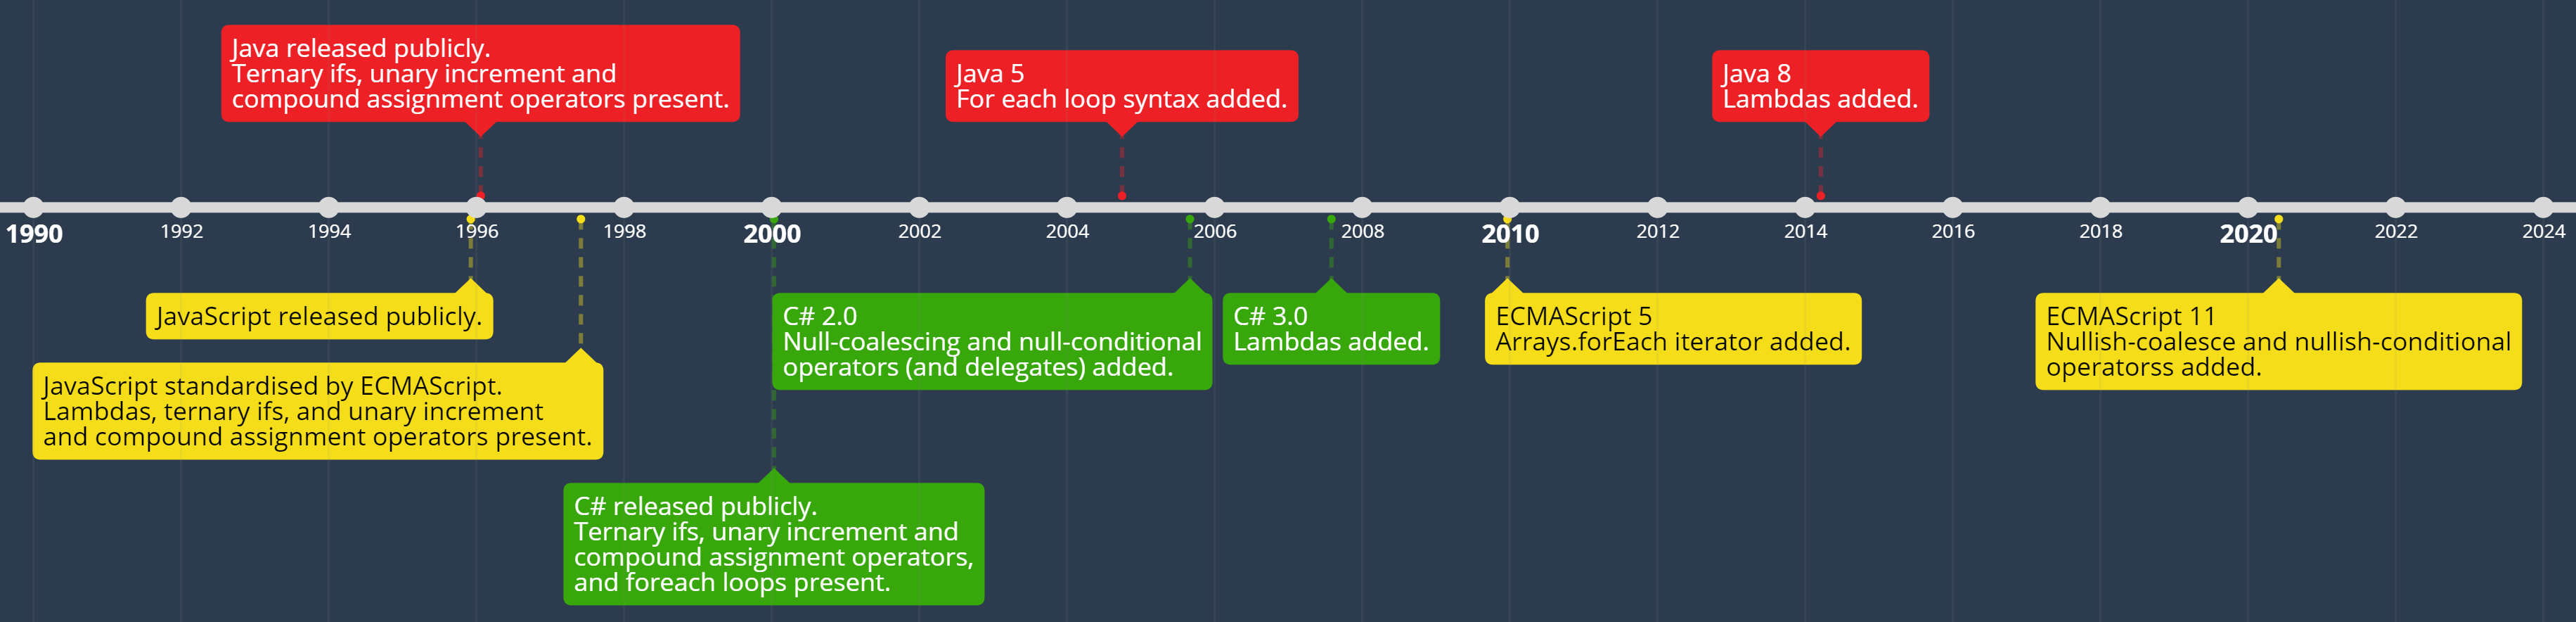
\includegraphics[width=1.5\textheight]{timeline}
        \caption{Timeline of the addition of advanced constructs to three modern languages.}
        \label{fig:timeline}
    \end{figure}
\end{landscape}
\newpage
\section{Study Design}
    \subsection{Survey}
    \label{subsec:survey}
        One of the facets of this study was to capture and analyse the perceptions and thoughts of a number of professional software developers with regard to the constructs being examined.
        
        This was carried out using a survey, constructed following guidelines laid down by both published literature (\cite{goodSurveys1}, \cite{goodSurveys2}) as well as a small amount of grey literature provided by higher education bodies. This allowed better questions to be written, that ensured they were no longer than necessary, used no double negatives, were not leading questions, only attempted to address one issue, and were not too vague. The design was also guided by these sources to include at least one open-ended question to allow participants to put forward any exceptional or unexpected information that could prove highly valuable to the study. Rightfully, notable mention is made at all stages to use of appropriate moral and ethical frameworks. In this instance, very little in the way of any problematic material is examined. The most personal question asked in the survey is how many years participants have been programming for - no other questions of a remotely personal nature are asked.

        Using the Qualtrics platform also allowed the usability of the survey to be examined by the Qualtrics' inbuilt system. This advised the design of the survey to be as easy to use as possible, increasing the likelihood of respondents completing their submissions. The only exception to this was the use of matrix table questions, which are not particularly friendly to mobile users. Despite this, they were used as they provided the best and most concise way to display the literal matrix of options available due to the presence of multiple constructs the question pertains to. Figure \ref{fig:matrixTable} shows one such question. The full survey is available in Appendix \ref{apx:survey}
        
        \begin{figure}[htbp]
            \centering
            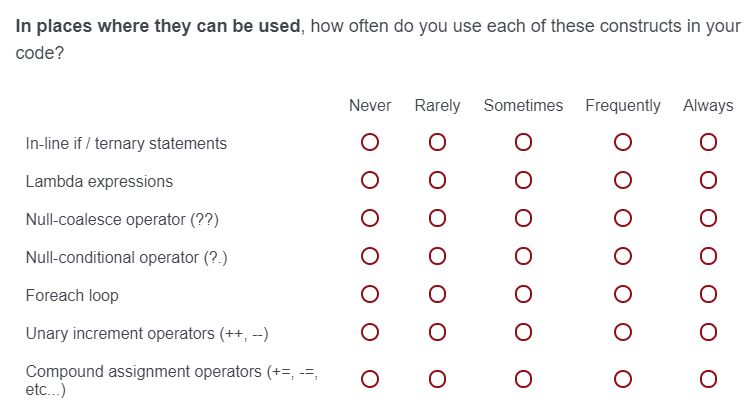
\includegraphics[width=0.8\textwidth]{matrixTable}
            \caption{A matrix table question used in the survey.}
            \label{fig:matrixTable}
        \end{figure}

        \subsubsection{Questions}
        \label{subsubsec:surveyQuestions}
            Prior to designing, it was established that the survey must be able to provide insight that may help to answer the following questions:
            \begin{enumerate}
                \item Are the participants \emph{aware} of the constructs?
                \item Do the participants \emph{use} the constructs?
                \item Are participants \emph{encouraged to use} the constructs?
                \item Do the participants think these constructs are better for:
                \begin{enumerate}
                    \item brevity?
                    \item clarity?
                    \item code efficiency/performance?
                \end{enumerate}  
                \item Do the participants think that the constructs are better used in some languages than in others?
                \item Do participants rewrite code \emph{to use} or \emph{to not use} the constructs?
            \end{enumerate}
            
        \subsubsection{Participants}
            A convenience sample of participating developers was recruited from within the Information Systems Services department (ISS) within Lancaster University by means of a blanket email sent out to all teams and filtered down via regular communications channels within the department. This gathered 40 responses in total, 23 of which completed the survey and may be considered valid responses.
            
            Due to the distribution method, there is no guarantee that all respondents are software developers by profession, however, all participants had a minimum of one year of programming experience, nearly half falling into the 1-4 years of experience category, with three participants having between 10 and 14 years experience and the remaining 8 having over 20 years of experience. This statistic was the only personal data collected and does not identify participants.
        \subsubsection{Questions}
            The survey was created using Qualtrics, as provided by Lancaster University, and consisted of a maximum of 16 questions and a minimum of 2 questions (depending on certain answers).
            Participants were first asked to indicate which of the constructs they were aware of so that only questions and option relating to those constructs they were aware of were shown to them. For each construct they were of, participants were asked to a series of questions design to address the questions listed in Section \ref{subsubsec:surveyQuestions}, focussing on: frequency of use, reasons to and to not use each construct, perception on code performance, and perception of industry-wide usage per-language.
            
            Lastly, participants were asked if they had any further comments, which invited some very interesting points that will be discussed alongside the rest of the results in Section \ref{subsec:results}.
    \subsection{Static Code Analysis}
        Static code analysis is concerned with checking programs and code for errors without the need to actually execute it. That is, a static code analysis tool will read the source code (or the compiled intermediary language in some cases), construct some form of abstract model of the program and then run a series of tests (often pattern-matching in nature) to detect well-known possible pit-falls, bugs, and problems \cite{staticCodeAnalysis}.

        These tools will often make recommendations on how source code may be improved in numerous way beyond explicit bugs and problems, such as stylistic improvement that make use of advanced syntax whatever given language is being analysed - advanced syntax akin to the constructs being examined here. Accordingly, static analysis tools were employed to investigate whether or not they made any recommendations for or against any of the constructs in question. SonarQube and Semgrep were selected for this purpose as they both support all three languages being subject to analysis, they are both under recent, active development, and because they both have free variants. Both tools were run against sample control code files and large open source repositories in the earlier mentioned three languages: C\#, JavaScript, and Java.
            
        \subsubsection{Sample Code Files}
            The sample code files were created to act as a baseline or control test to see if SonarQube or Semgrep made any note at all about the bare use and/or inclusion of any of the constructs.

            Each file contains a bare (non-contextualised) example of each of the constructs placed directly alongside their `simple syntax' functionally equivalent counterparts. Each file is valid syntax for its language, and all of them may be executed, though none of them have a true entry point or way to actually \emph{run} the code within itself - the functions and methods are present purely to \emph{be present} so that they may be analysed by SonarQube and Semgrep. Though there are differences between the three languages, the form of the sample code was kept as similar as possible to preserve their purpose as control samples, without adding deliberately unusual syntax that may contaminate the output of SonarQube and Semgrep.
        \subsubsection{Open Source Repositories}
            Four large, open source code repositories were selected from GitHub to be analysed for this study, one each in C\# and JavaScript, and two in Java. The selection process was simple: 
    \subsection{Git Commit Analysis}
        To supplement the static analysis of the repositories, manual, by-hand analysis of the commits made to these repositories was also undertaken.

        The goal of this branch of the study was to understand if and how standards are being maintained within the repositories within reference to the constructs and to general style-keeping. This was carried out by cloning the repository and examining the commit history using \codeword{git log}. A list of keywords were run against the commit history using the \codeword{--grep=<pattern>} option to \codeword{git log}. The keywords used are listed below:
        
        \begin{center}
            \begin{tabular}{ | l | l | }
                \hline
                \textbf{General} & style \\
                \hline
                \textbf{Ternary} & ternary, conditional, \codeword{?:}, elvis \\
                \hline
                \textbf{Null coalesce/conditional} & null, coalesce, conditional, \codeword{??}, \codeword{?.}, \codeword{?[} \\
                \hline
                \textbf{Lambda} & lambda, arrow, \codeword{=>}, \codeword{->} \\
                \hline
                \textbf{For each} & foreach, for each \\
                \hline
                \textbf{Unary Operators} & unary, increment, decrement, ++, -{}- \\
                \hline
                \textbf{Compound Operators} & compound, assign, \codeword{+=}, \codeword{-=}, \codeword{*=}, \codeword{/=}, \codeword{|=}, \codeword{&=} \\
                \hline
            \end{tabular}
        \end{center}

        Some of these keywords generated cross-over between those meant to highlight changes around a particular construct, but this was unimportant as these keywords were only used to create a list of  `interesting' commits. Commits were deemed interesting if the commit message and/or description contained reference to any of the keywords in such a way that it seem plausible that a change was made regarding any relevant construct. For each commit in the resultant list, the changes were scrutinised closely to pick out changes made that: added, removed, altered, or commented on use of any of the constructs. Each type of change was documented and counted per commit.

\newpage
\section{Results}
    \subsection{Survey}
    \label{subsec:results}
        As described in Section \ref{subsec:survey}, a survey was conducted with experienced professional software developers and programmers. This revealed interesting patterns of usage (or lack of usage) of the constructs, and some interesting perceptions that may prove useful in future research focussed on performance and use in the wider industry.

        The following sections will detail the results of the survey, including threats to the usefulness of the survey and the patterns discovered by the survey. All percentage values given have been rounded to 1 decimal place.
        \subsubsection{Threats to Survey}
            As mentioned in the introduction, the survey participants were only a convenience sample of developers. This means that the results may not be generalised very easily to a wider group of developers. The results may be generalised \emph{within} ISS but not outside. Further research and more significant surveying should be undertaken to verify if the results found within ISS may be applied to a wider populace of developers.

            Despite this, a survey still provides a very quick and  easy way to gather information from a sample size much larger than would be trivial than many other methods.
        \subsubsection{Awareness}
            Awareness of the constructs was gathered by a simple multiple choice question with a binary yes/no for each. Participants could indicate whether or not were familiar with all, some, or none of the constructs.
            \\\newline
            All participants were aware of unary operators and ternary/in-line if-statements, nearly all were aware of compound operators and lambdas, and most were aware of null-coalesce and null-conditional. Figure \ref{fig:awareness} shows these results in a graphic format.

            \begin{figure}[htbp]
                \centering
                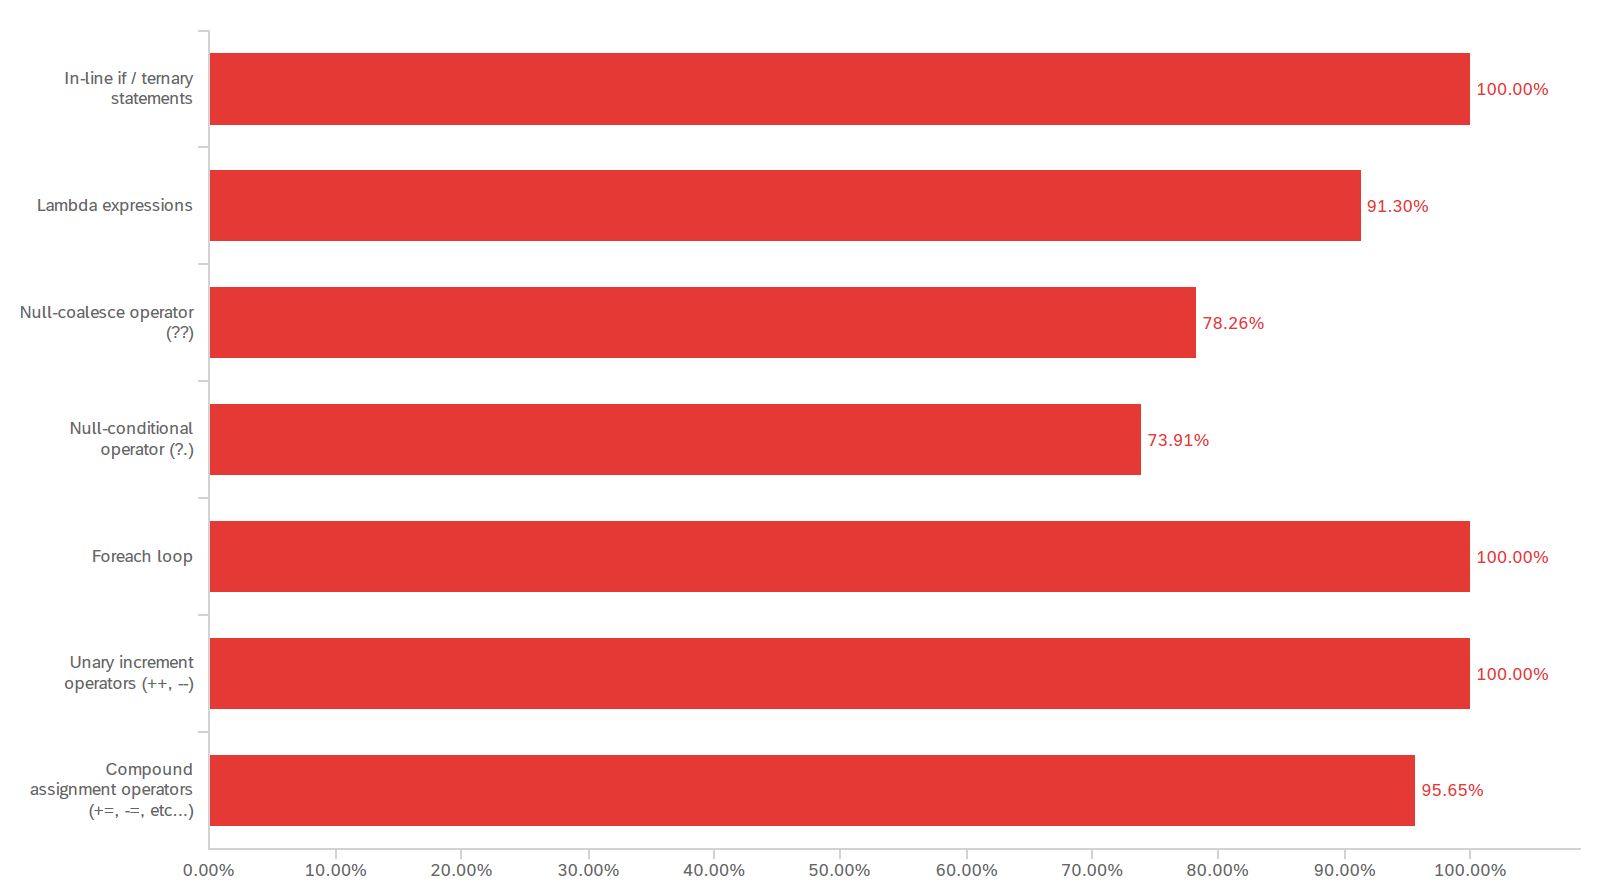
\includegraphics[width=0.8\textwidth]{awareness}
                \caption{Percentage of participants aware of each construct}
                \label{fig:awareness}
            \end{figure}

            The most stand-out piece of information here is that the \emph{absolute} awareness of the null-coalesce and -conditional operators was markedly higher than might be expected. This can likely be attributed to the fact that participants were all from within ISS, where the  technology stack contains a significant amount of C\#, in which these operators are often seen. If the survey were repeated over more diverse and broad range of developers working in more varied technology stacks (for example, those focussed much more on Java, or C/C++), it is reasonable to assume that awareness of these operators would be less. This is a trend that is repeated elsewhere in the results set.
            It is also of note (if not significantly so) that not \emph{all} participants were aware of compound assignment operators, whereas all participants \emph{were} aware of ternaries - a ranking inverse to what was expected. However, the difference in the numbers are not statistically significant, comprising no more than one or two responses. To draw any conclusion from this datum would require it being replicated in a greater sample set.
        \subsubsection{Frequency of Use}
            To assess how often participants use each of the constructs, they were asked specifically: \textit{In places where they can be used, how often do you use each of these constructs in your code?}, that is, ``for every chance you \emph{could} use the construct, how often do you?''
            \\\newline
            It was the extreme ends of the scales in this question that provided the most interesting results here. Firstly, and perhaps reassuringly, only one data point was recorded, for any construct, under the `never' option, with just one respondent indicating that they never use the null-coalesce operator. Conversely, `for each' was the most selected construct in the `always' category, with 44\% of participants selecting this option, followed closely by compound assignment operators at 41\%.

            Across all constructs, the majority of responses fell into the `frequently' category, holding 39\% of the total selections, with the `sometimes' category at 27\%. This general erring toward the more frequent end of the scale holds not only for the collective dataset but also for each construct when examined individually, as may be seen in figure \ref{fig:freqUse}

            \begin{figure}[htbp]
                \centering
                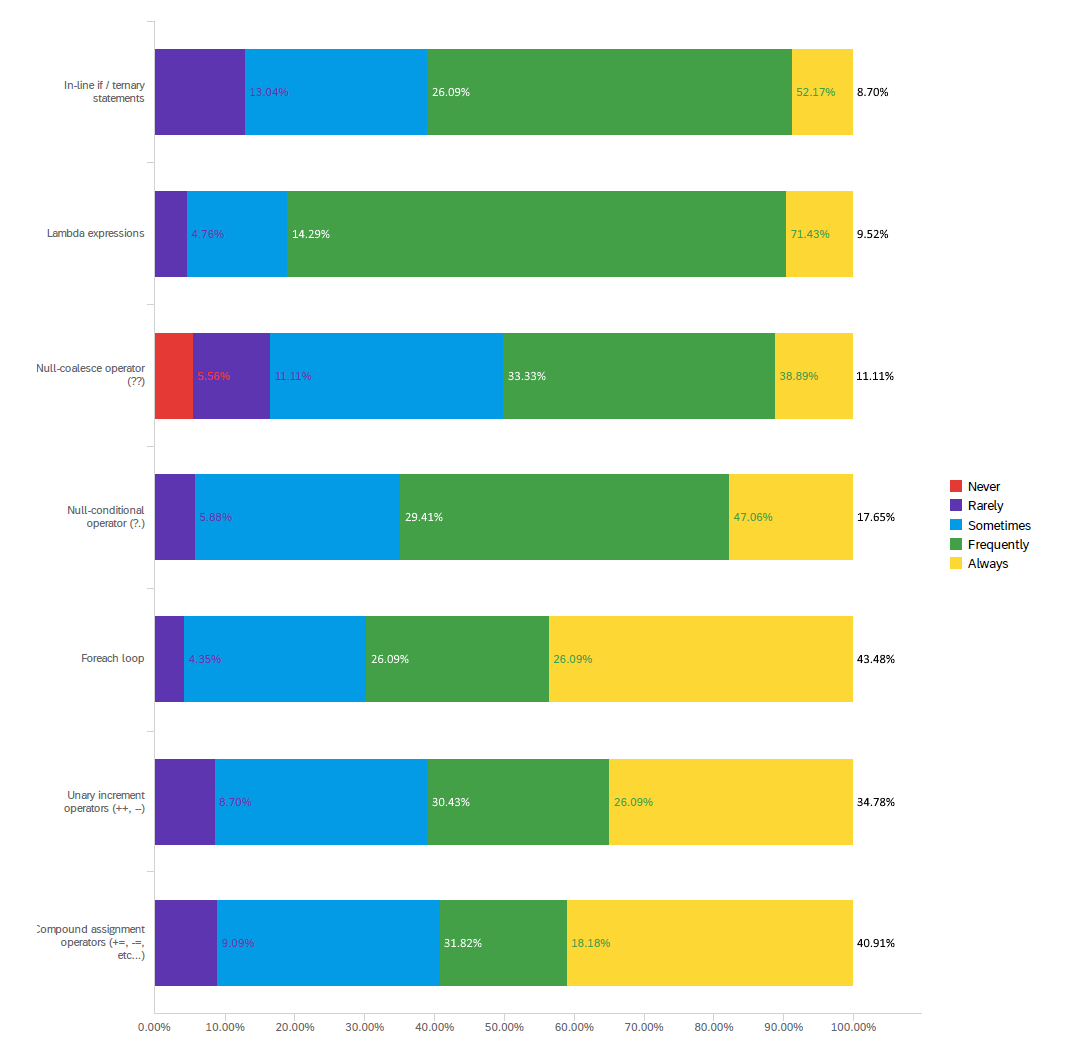
\includegraphics[width=0.9\textwidth]{freqUse}
                \caption{Frequency with which participants said they used advanced constructs, grouped by construct}
                \label{fig:freqUse}
            \end{figure}

            As is visible in figure \ref{fig:freqUse}, the use of lambdas in moderation is the most agreed upon data point here, with just over 70\% of responses labelled `sometimes' for lambdas. This is likely explainable by a variety of reasons, not least is the fact that lambdas are very powerful and complex structures, much more so than the other constructs being studied, and as such, the number of situations where they \emph{can} be used likely greatly exceeds the number situations where they \emph{should} be used. This distinction around lambdas becomes more apparent in later questions.
            Of note, again, the results for the null-coalesce and null-conditional operators. Although the numbers of participants familiar with these operators is fewer, those that were aware of them do not shy away from them, using them with comparatively similar frequency to the other constructs.
        \subsubsection{Reasons To Use}
            Participants were then asked to indicate \emph{why} they chose to use each given construct. The four options were presented:
            \begin{itemize}
                \item ``It is company style''
                \item ``It makes code clearer''
                \item ``It makes codes simpler''
                \item ``It makes code run faster''
            \end{itemize}
            All, some, or none of the options may have been selected. Where the exclusive option ``None of these'' was selected, participants were prompted to give their own reason.
            \\

            The trend here was extremely clear: the most common reasons for using any of the constructs was for clarity and simplicity. ``It makes code clearer'' and ``It makes code simpler'' took 39.4\% and 42.3\% of all selections made respectively. The data for the selections totalled across each construct is shown in Figure \ref{fig:toUsePie}.

            \begin{figure}[htbp]
                \centering
                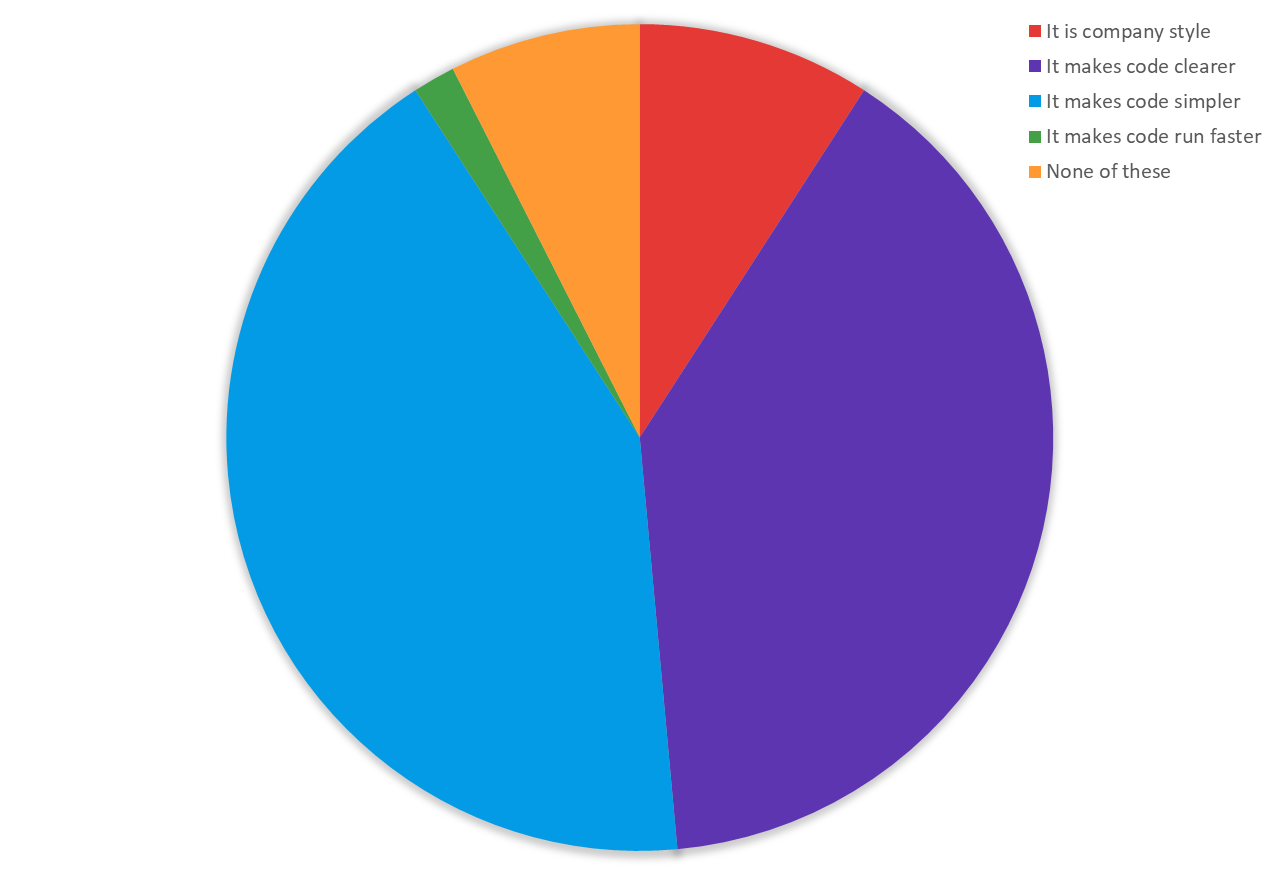
\includegraphics[width=0.9\textwidth]{toUsePie}
                \caption{Reasons to use constructs, totalled across all constructs.}
                \label{fig:toUsePie}
            \end{figure}

            Six participants selected `None of these' for at least one construct, two of whom selected this option for all constructs they were aware of and both instead said that they choose to use the constructs based on personal preference or habit. Another two selected this option for lambdas alone, one saying that they are aware of don't use lambdas, and the other highlighting a possible flaw in this study regarding lambdas. The participant noted that there are places where ``there is no rational alternative to using a lambda expression. It does not make the code simpler or clearer, it's just \textbf{necessary} to use a lambda.'' This brought to attention the fact that lambdas may be a more functional language feature, not fitting with the other constructs here. This is discussed further in Section \ref{subsubsec:lambdas}.
            One participant also said that they would generally use `map' instead of a \codeword{foreach} loop, claiming ``it helps avoid `off by one' errors''. Off-by-one-errors occur when iterating over an array or other list of \textit{m} through \textit{n} items. Asking how many items there are (how many loop iterations are required), the intuitive answer of \textit{m} - \textit{n} is incorrect, the correct answer being (\textit{m} - \textit{n}) + 1. This is illustrated using a specific type of off-by-one error, a \textit{fencepost error} in Figure \ref{fig:fencepost}.
            \begin{figure}[htbp]
                \centering
                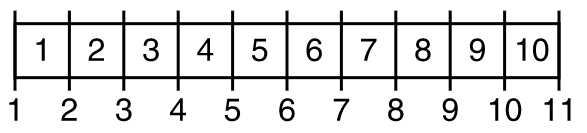
\includegraphics[width=0.5\textwidth]{fencepost}
                \caption{If you have a fence with 10 posts, how many bounded sections exist between the posts? The intuitive answer is 10, but it is in fact 11. This is a specific off-by-one error.}
                \label{fig:fencepost}
            \end{figure}

            It is not clear what advantages a `map' function has over a \codeword{foreach} loop to avoid off-by-one errors. In fact, conventional wisdom dictates that \codeword{foreach} loops, by nature should, avoid these errors by virtue of the fact that they\emph{remove} the need for a programmer to calculate the necessary number of loop iterations. It is plausible to suggest that this response was given by mistake, instead meaning to refer to traditional \codeword{for} loops, rather than \codeword{foreach} loops.
            \begin{figure}[htbp]
                \centering
                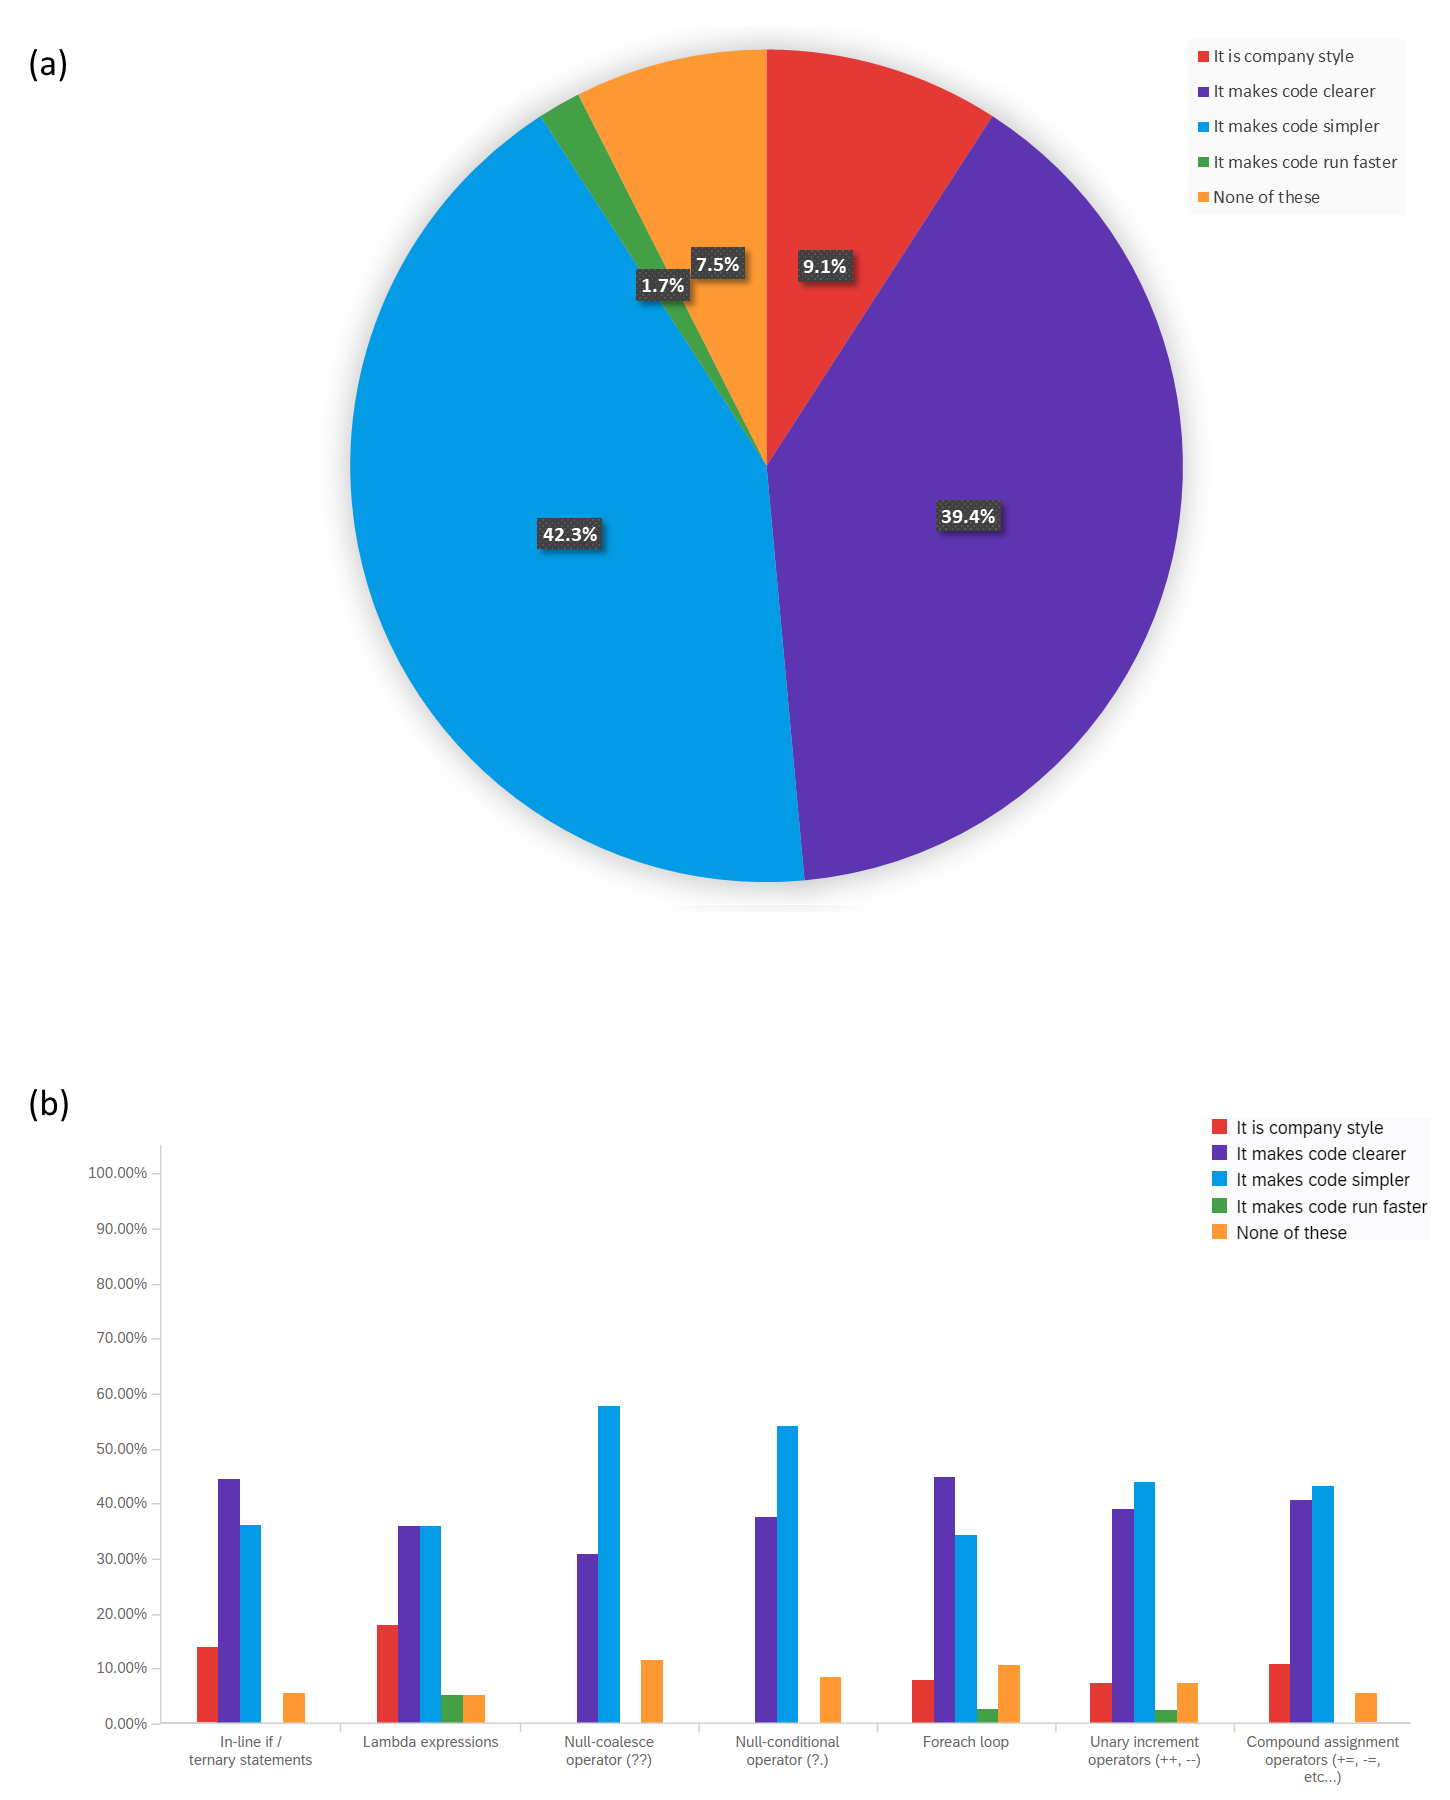
\includegraphics[width=0.9\textwidth]{toUse}
                \caption{Reasons to use constructs grouped by construct. Figures normalised to percentages per construct.}
                \label{fig:toUse}
            \end{figure}

            Figure \ref{fig:toUse} part repeats the data above, again showing that clarity and simplicity are the most common reasons. We can also see that the split is \emph{mostly} even between these two reasons, null-coalesce being a slight exception, with nearly double as many responses selecting simplicity over clarity. Null-conditional follows this pattern, but the difference is less pronounced.
            Other notable statistics are: no participants said that they used null-coalesce or -conditional due to company style, and the three constructs that had code run speed selected. Two participants selected this for lambdas, and one each both selected this for \codeword{foreach} loops and unary operators. These are statistically insignificant, but it is still of note that none of the other constructs had any selections regarding faster code running.
        \subsubsection{Reasons To Not Use}
            To provide the other half of the story to the previous section, participants were also asked about the reasons they choose to \emph{not} use the constructs. Similar to before, the options presented were:
            \begin{itemize}
                \item ``It is company style''
                \item ``It would make code less clear''
                \item ``It would make code more complex''
                \item ``It would make code run slower''
            \end{itemize}
            With an additional ``None of the above'' option, selection of which reveals an additional question for participants to again give their own reason.
            \\

            Reasons of clarity and complexity were the most selected again, with 48.2\% of all selections attributing maintaining the clarity of code as a reason to not use a given construct, and complexity at 23.9\%. More than double the proportion of selections were present for ``None of these'' compared to the when asked for reason \emph{to} the constructs - here, 16.2\% of selections were placed here. The reasons provided by these respondents were quite varied but very interesting and are all worthy of discussion:

            \begin{itemize}
                \item Personal preference
                \begin{itemize}
                    \item Mentioned explicitly by three, and implicitly by one, of the ten individuals who gave their own reasons.
                    \item One noted that ``as long as code is well documented you can use any of them''.
                    \item One wrote that there is no company style for these constructs and that there is instead guidance on larger/less granular things like examples of a model class. This is contradicted by other responses, though it's plausible the two are subject to different standards.
                    \item The third, the only of the ten that overlap with those that selected this option on the previous question. Simply stating that it is personal preference.
                    \item The final reason links usage of compound of unary operators goes against their preference to use a `functional style' and to `avoid mutability of variables'. This raises interesting questions about the use of functional programming ideas in non-functional paradigms.
                \end{itemize}
                \item `I [almost] always use this construct'
                \begin{itemize}
                    \item Two participants said they would always use unary increment operators
                    \item One said they would always use compound operators
                    \item Another said the only time there would not use null-coalesce/null-conditional is when null checking is not required
                \end{itemize}
                \item Other/Unqualified
                \begin{itemize}
                    \item One participant stated that a \codeword{for} loop may be preferable to a \codeword{foreach} loop when the index variable is needed. They then go on to say that it also `depends how I'm feeling'.
                    \item Regarding lambdas and unary and compound operators, one participant said: ``sometimes these operators don't account for requirements such as type checking or formatting'' without any more description.
                    \item One participant claimed that \codeword{foreach} loops may introduce errors, but did not explain further.
                \end{itemize}
            \end{itemize}

            \begin{figure}[htbp]
                \centering
                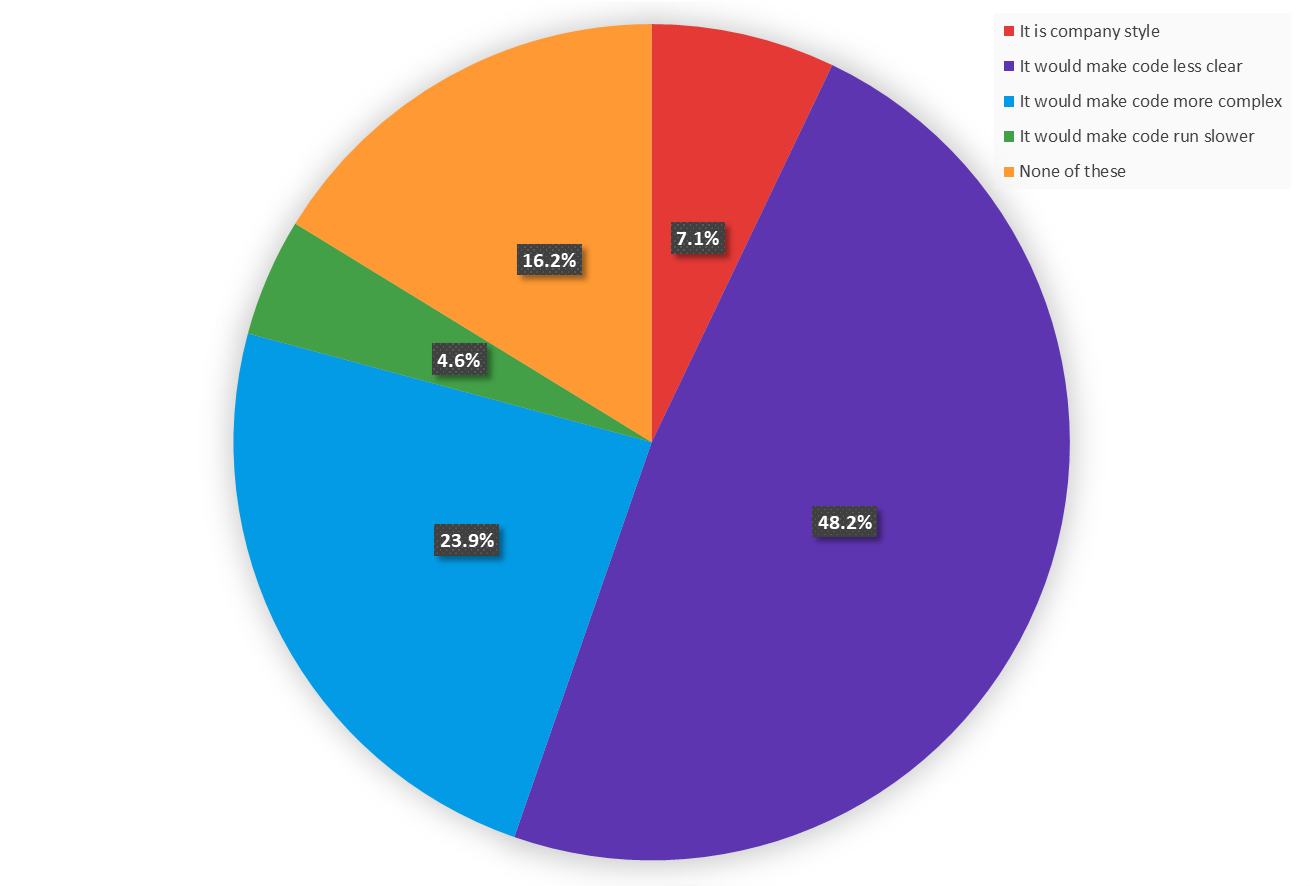
\includegraphics[width=0.9\textwidth]{toNotUsePie}
                \caption{Reasons to not use constructs, totalled across all constructs.}
                \label{fig:toNotUsePie}
            \end{figure}

            Only 4.5\% selected ``It would make code run slower'' - logically, this would make sense factually too, as most of these constructs are plain syntactic differences that, with most modern compilers and interpreters, are likely to produce the same bytecode and/or machine code. Lambdas and \codeword{foreach} are likely the only exceptions to this. The former has other potential implications beyond just how it looks on-screen, the latter (depending on language) may be a change from an array index to initialising an iterator and calling on that instead. This is reflected in the thoughts of participants in Figure \ref{fig:toNotUse}, showing that these two constructs were the only two to have received the selection pertaining to code run speed.

            \begin{figure}[htbp]
                \centering
                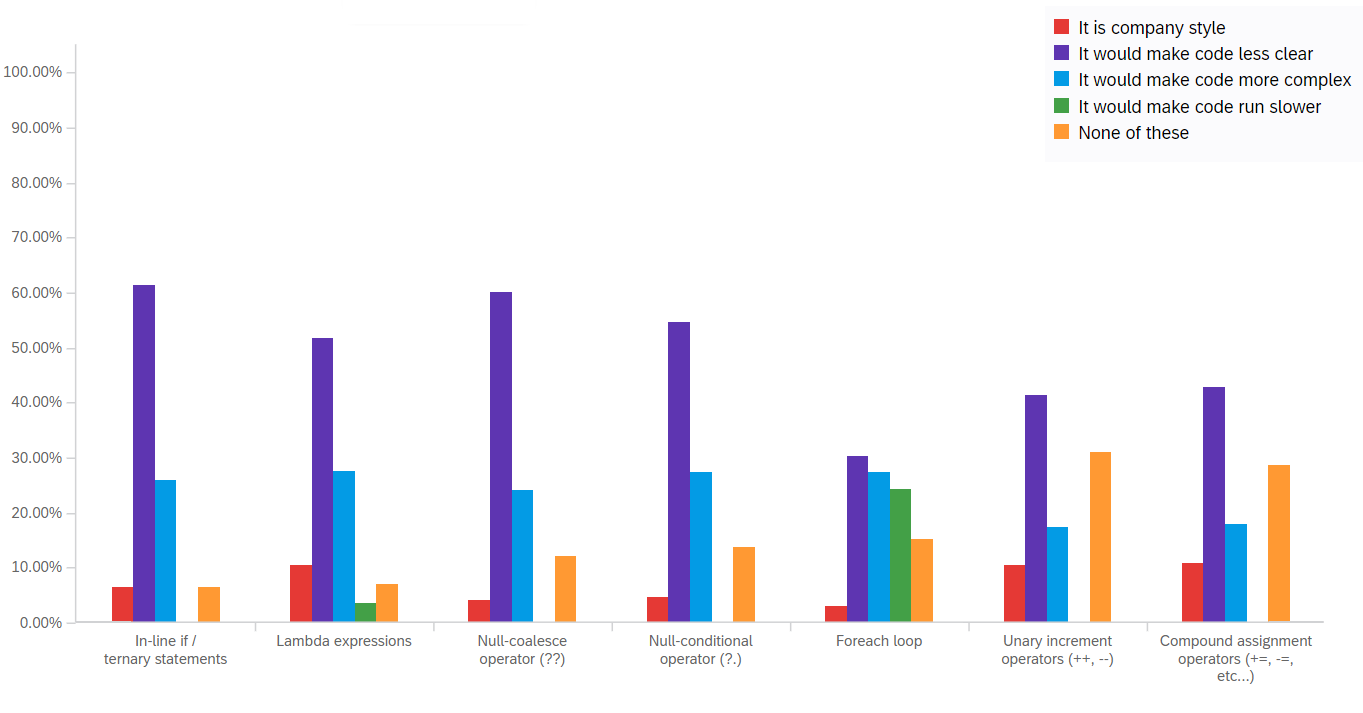
\includegraphics[width=0.9\textwidth]{toNotUse}
                \caption{Reasons to not use constructs grouped by construct. Figures normalised to percentages per construct.}
                \label{fig:toNotUse}
            \end{figure}

            The breakdown in Figure \ref{fig:toNotUse} also confirms that clarity was the most common reason selected by a wide margin for four of the constructs, but not for unary and compound operators (multiple reasons, described above) and 
            for \codeword{foreach} loops (run speed was a concern as described immediately above).
            All constructs had a small number of responses claiming company style as reasons for not using them, but this is a relatively small number compared to the proportion that cited clarity or complexity or their reason.
        \subsubsection{Performance}
            []
        \subsubsection{Usage In Wider Industry}
            []
    \subsection{Static Code Analysis}
        []
        \subsubsection{Sample Code Files}
            Bugger all picked up, tools do not care
            \begin{itemize}
                \item Picked up basic \codeword{for} in place of JS \codeword{for-to} (not \codeword{for/each})
            \end{itemize}
        \subsubsection{Real-World Code Bases}
            []
\newpage
\section{Conclusion}
\label{sec:conclusion}
    []
    \subsection{Review of Aims}
        The following list repeats the aims presented at the start of this report, with each aim followed by an overview of relevant results obtained.
        \begin{itemize}
            \item \textcolor{gray}{\textit{[]}}
                []
            \item \textcolor{gray}{\textit{[]}}
                []
            \item \textcolor{gray}{\textit{[]}}
                []
            \item \textcolor{gray}{\textit{[]}}
                []
            \item \textcolor{gray}{\textit{}}
                []
        \end{itemize}
    \subsection{Reflections}
        []
        \begin{itemize}
            \item survey: what does "complexity" mean? Computational? That'd be covered by slow/faster?
            \item GitHub repo selection: mistakenly thought it was `top of all repos for lang., it was not. (Check Tracy emails for reference and remedy, time permitting)'
            \item Use/Not Use, discrepancy in tense used in presented options, potentially created a bias toward `use', although this would have bene introduced AFTER the `use' question (participants can step backward through survey however)
        \end{itemize}

        \subsubsection{Lambdas}
        \label{subsubsec:lambdas}

        
    \subsection{Negative Impacting Circumstances}
        The on-going coronavirus pandemic is still very much a factor in the lives us all. :(
    \subsection{Future Research}
        []
    \subsection{Closing Statement}
        []

\newpage
\bibliography{ref}
\newpage
\section*{Appendix}
    \subsection*{A: Project Proposal}
        \includepdf[pages=-]{../Ref/proposal}
    \subsection*{B: Survey}
    \label{apx:survey}
        \includepdf[pages=-]{../Ref/survey}
\end{document}